\chapter*{Introduction}
\addcontentsline{toc}{chapter}{Introduction}
\label{chap:intro}



Concurrent systems are a particular framework where different agents or processes evolve in the same environment. They must cohabit by managing the resources, avoiding conflicts. Verifying such programs is a difficult task: it is necessary to ensure that the system never goes wrong, regardless of its behaviors. One could apply classical methods from sequential systems, by checking every possible execution of the system, that is what is used in \emph{interleaving} semantics for concurrency. However, the number of such executions grows exponentially with the size of the system, which make this method unpractical. 

The idea of \emph{true concurrency} is that several executions may have exactly the same behaviors because, for each agent, they correspond to the same execution, differing only by the way they are scheduled one from each other. This suggests that one should study not every possible execution, but every possible execution modulo an equivalence relation, relating executions that are only differing by permuting independent actions, which decreases greatly the number of execution to consider.

Surprisingly, the models for true concurrency are very geometric by nature: they have algebraic structure which can be interpreted topologically. Roughly speaking, such a system is a topological space of states, where executions are interpreted as ``monotonous'' (more precisely, \emph{directed}) paths in this space, following the execution flow of the system. The equivalence relation on executions is then interpreted continuously: two executions, seen as directed paths, are equivalent if one can be continuously deformed into the other while preserving the direction of times, the execution flow.

This brings the idea that those models for true concurrency must be studied geometrically using tools from mathematics. Moreover, studying spaces, paths and continuous deformations of paths is one of the main ideas of a well known field in mathematics: algebraic topology. Intuitively, its goal is to study spaces up to continuous deformations using algebraic structures (categories, groups, modules, ...) that reflect the geometry of the space: paths, continuous deformations of paths, continuous deformations of continuous deformations, and so on.

The only difference with our study of truly concurrent system is the crucial role of the direction from execution flow. Everything should be compatible with this structure: paths must be directed, deformations must be in some way directed, and so on. This opens a new field of research: \emph{directed algebraic topology}, where the main focus is to construct similar algebraic invariants for spaces with direction, defining suitable notions of deformations that are compatible with direction, and so on.


\section*{True concurrency}

The models for true concurrency were designed by extending the classical models of transition systems for interleaving semantics. The idea is to specify somehow that some actions are independent and can be done in any order, and in particular, \emph{simultaneously}. A typical example is two agents $A$ and $B$, making some computations and updating the value of some variables. For example, assume that there are two different variables $X$ and $Y$ and that $A$ wants to update the value of $X$ to $0$, noted $X := 0$; $B$ wants to update the value of $Y$ to $1$, noted $Y := 1$. With a classical transition system, this concurrent system would be modeled as follow:
	\begin{figure}[H]
		\begin{center}
    			
\begin{tikzpicture}[scale=1]
		
	\node (1) at (0,0) {$q_\varnothing$};
	\node (2) at (3,0) {$q_A$};
	\node (4) at (0,3) {$q_B$};
	\node (3) at (3,3) {$q_{A,B}$};
	
	\path[->,font=\scriptsize]
		(-0.5,-0.5) edge (1)
		(1) edge node[below]{$X := 0$} (2)
		(1) edge node[left]{$Y := 1$} (4)
		(2) edge node[right]{$Y := 1$} (3)
		(4) edge node[above]{$X := 0$} (3);
			
\end{tikzpicture}


  		\end{center}
	\end{figure}
With this model, the different possible behavior are first $A$ does its action then $B$ or first $B$ does its action then $A$, and those two behaviors are considered independently. However, with the idea from true concurrency, since $A$ and $B$ are updating different variables, there is no conflict or concurrence on the resources (here the variables). So, those two actions can be considered independent, meaning that doing first one then the other or in the other way makes no difference. Furthermore, those two actions can be made simultaneously. 

There are several way to specify that actions are independent:
\begin{itemize}
	\item the first basic idea is to define a relation directly on transitions depicting the fact that  they are independent. This leads to the notion of \emph{transition system with independence} \cite{nielsen94}.
	\item the second idea is to regroup transitions that represent the same event. In the previous example, the two transitions labelled $X := 0$ represent the same event ``$A$ update the value of $X$ to $0$''. One can then define an independence relation on those events, this leads to the notion of \emph{asynchronous systems} \cite{shields85,bednarczyk87}.
	\item the last is to specify squares of transitions of the form:
	\begin{figure}[H]
		\begin{center}
    			\begin{tikzpicture}[scale=1]
		
	\node (1) at (0,0) {$\bullet$};
	\node (2) at (3,0) {$\bullet$};
	\node (4) at (0,3) {$\bullet$};
	\node (3) at (3,3) {$\bullet$};
	
	\path[->,font=\scriptsize]
		(1) edge node[below]{$a$} (2)
		(1) edge node[left]{$b$} (4)
		(2) edge node[right]{$b$} (3)
		(4) edge node[above]{$a$} (3);
			
\end{tikzpicture}
  		\end{center}
	\end{figure}
	where $a$ and $b$ are independent actions and to add a formal square in the specification, depicted as follow:
	\begin{figure}[H]
		\begin{center}
    			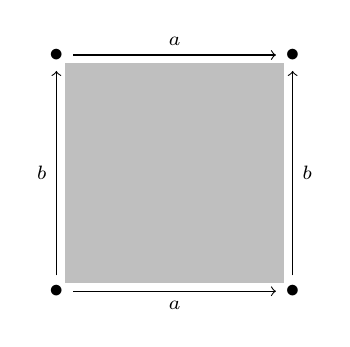
\begin{tikzpicture}[scale=1]
		
	\node (1) at (0,0) {$\bullet$};
	\node (2) at (3,0) {$\bullet$};
	\node (4) at (0,3) {$\bullet$};
	\node (3) at (3,3) {$\bullet$};
	
	\path[->,font=\scriptsize]
		(1) edge node[below]{$a$} (2)
		(1) edge node[left]{$b$} (4)
		(2) edge node[right]{$b$} (3)
		(4) edge node[above]{$a$} (3);
	
	\draw[draw = white, fill = gray!50] (0.1,0.1) rectangle (2.9,2.9);
			
\end{tikzpicture}
  		\end{center}
	\end{figure}
	
	 This idea can be extended to higher dimensional behaviors: one can specify $n$-dimensional cubes of transitions where parallel transitions are labelled by the same action, and all actions are independent to each other and add a formal $n$-dimensional cube in the specification. This leads to the notion of higher dimensional automata \cite{pratt91}, (HDA for short).
\end{itemize}

All those models come with a way to compare them, defined with bisimulations, extending the work from classical transition systems.


\section*{Modeling true concurrency with geometry}

HDA are very geometrical by nature. They are specified as formal elements of any dimension representing independent behaviors of actions. Those formal objects must satisfies some boundary conditions: if you consider a subset of $n-1$ actions among $n$ independent actions, then they must be independent. This allows one to interpret formal objects of dimension $n$ as a geometrical cube of dimension $n$ and the equations satisfied represent glueing conditions on those cubes. To summarize, from an HDA, it is possible to construct a topological space by glueing cubes together. This space represent the space of states of the HDA, and is called the \emph{geometric realization}. For example, the square depicted above can be geometrically interpreted as a real square $[0,1]\times[0,1]$.

From this geometric interpretation, one can see executions as paths, that is, continuous functions from the segment $[0,1]$ to the geometric realization. The only problem is the directedness: an execution in HDA is directed by nature. It has a source and a target, and the transition can only go from the source to the target. Geometrically, a transition is modeled as a copy of the segment $[0,1]$ inside the geometric realization, the source being mapped on $0$, the target on $1$. The problem is that paths in $[0,1]$ are not directed (here, in the sense they are not monotonic), and so one can define a path from $1$ to $0$. Those paths cannot be interpreted as executions in the underlying HDA. So one must specify somehow some directedness on the geometric realization: the cubes $[0,1]^n$ used to construct the geometric realization are naturally directed. One can define a partial order on them as the product ordering. This local ordering on each cube can be extended to a directed structure on the whole geometric realization:
\begin{itemize}
	\item either by following the idea from manifolds, that local orders which globally behave well. That leads to \emph{local po-spaces} \cite{fajstrup03} and \emph{streams} \cite{krishnan09},
	\item or by specifying a collection of paths that are locally monotonic. This leads to \emph{d-spaces} \cite{grandis01}.
\end{itemize}
Either way, this directed structure allows one to define \emph{directed paths}, which are paths that are compatible with the directed structure, and that will model executions.

Following the idea from true concurrency, executions of HDA can be related using an equivalence relation interpreting that executions equal up to permutation of independent actions. It is called \emph{homotopy} in \cite{vanglabbeek05}. Geometrically, this can be modeled using the notion of \emph{dihomotopy}, extending to a directed framework the notion of homotopy in topological spaces. Homotopy is the equivalence between paths of a space, relating paths that can continuously be deformed one from the other. Similarly, dihomotopy is the relation that relates two directed paths that can continuously deformed one from the other, in such a way that the deformation must be somehow compatible with directedness.


%HDA very geometric, geometric realization, point = state, directed paths = executions, continuous deformations of directed paths = equivalence of executions up to rearrangement of independent actions

\section*{Directed algebraic topology}

Spaces, paths, homotopies are studied in the so called field of \emph{algebraic topology}. In algebraic topology, one studies spaces modulo continuous deformations, called \emph{homotopy equivalences}. One can then construct algebraic invariants of homotopy equivalence: for example, paths modulo homotopy can be seen as the morphisms of a category, called the \emph{fundamental category}, which is an invariant modulo equivalence of categories. More generally, higher order deformations (much as, continuous deformations between homotopies) provides group structures, called \emph{homotopy groups}, which are invariants of homotopy equivalence. The problem with these algebraic invariants is that they are not easily computable. Other algebraic invariants were defined, extending the work on Euler characteristic: homology groups are Abelian groups that compute the number of ``holes'' of any dimension of a space. Those homology groups are computable. Although not complete, they are sufficiently precise in many cases.

The goal of \emph{directed algebraic topology} is to extend this work on directed spaces, defining directed analogue of homotopy equivalence, homotopy groups and homology groups, and so on. The most notable work is the one from Grandis, compiled in the textbook \cite{grandis09} where all those constructions were done for a specific notion of directed homotopy equivalence. This work, however, fails to describe some behaviors that we would be interested for our study of truly concurrent systems. 

Another thread can be found in \cite{fajstrup16}, compiling 20 years of work of the authors. Notably, their work on trace spaces (a nice abstraction of the notion of execution in this context) and on directed components (extending the work on the fundamental category and path-connected components in a directed setting), was a solid basis for this thesis. 

Another aspect is the work on model structures. Model structures are an abstract model for thinking about objects up to homotopies. The most known result on this subject \cite{nlabhh} is that the algebraic structure of topological spaces (with paths, homotopies, higher homotopies) can be reflected exactly by $\infty$-groupoids, that is, higher categories with objects, morphisms between objects, morphisms between morphisms and so on, where everything is invertible. This result is called the \emph{homotopy hypothesis}. Porter made some development on the same ideas in the directed case, in \cite{porter08,porter15}, looking for a model structure for d-spaces through the theory of $(\infty,1)$-categories.


\section*{Outline}

This thesis will focus mainly on the last aspect: constructing a coherent theory of homotopy equivalences and algebraic structures modeling homotopy and homology in the context of directed algebraic topology. The thesis will be structured in three parts.

\begin{itemize}
	\item[I)] In a first part, we will recall the models of true concurrency, either abstractly, or geometrically. In Chapter 1, we will investigate the abstract models extending transition systems: asynchronous transition systems, transition systems with independence and higher dimensional automata. We will study their bisimulations, namely, the ways to compare the behaviors of those systems. In Chapter 2, we will look at the geometric models. We will define the geometric realization and see an overview of the different way to add directedness on it. We will then see how states, executions, equivalence of executions modulo permutation of independent actions can be modeled geometrically. Finally, in Chapter 3, we will investigate the general notion of bisimilarity seen in Chapter 1, defined using lifting properties. This chapter will be independent of the rest of the thesis, and no particular focus on true concurrency and geometry will be made. For this bisimilarity, we will study a general class of models for which several equivalent characterizations hold. We will also see that a general notion of unfolding can be defined in this context.
	\item[II)] In the second part, we will focus on the homotopy theory of directed spaces. In Chapter 4, we will see two notions of directed homotopy equivalences proposed in \cite{grandis09}, the reversible and the directed one. We will see how they fail to capture some behaviors that we may want. We will also see what are their actions on the fundamental category and in what way this category is an invariant in terms of localizations. Finally, we will see a construction similar to the category of components from \cite{goubault07}, which is in between the fundamental category and its groupoidification and which is much more convenient for our study. In Chapter 5, we will investigate the homotopy hypothesis and its possible extension to the directed case. We will see that the idea from \cite{porter15} to compare homotopy theory of directed spaces to $(\infty,1)$-category is convenient when considering reversible equivalence, not more. We will then see how this can be slightly modified to take into account what reversible equivalence lacks, in particular using the category of components. Finally, we will design a notion of directed homotopy equivalence, the \emph{inessential equivalence} based on the idea of deformation retracts and of inessentiality from \cite{goubault07}. This inessential equivalence will have all the properties we expected: the category of components will be an invariant, it will be in between reversible and directed equivalences, and they allow a directed homotopy hypothesis.
	\item[III)] In the third part, we will focus on homology theories of d-spaces. In Chapter 6, we will look at the classical theory of homology in topological spaces and overview its particular interesting properties, in particular, the Eilenberg-Steenrod axioms \cite{eilenberg45}. We will then define our directed homologies, bimodule and natural homologies, following the idea that it must look at trace spaces and their evolution with time. Finally, we investigate the Eilenberg-Steenrod axioms for this homology. In Chapter 7, we define a notion of bisimilarity of diagrams, following the theory of \cite{joyal96}. We prove a few equivalent characterizations following the ones in classical bisimulations and we prove the decidability of the existence of such a bisimulation in a particular case. Finally, in Chapter 8, we use this notion of bisimulation to compare diagrams of homology and homotopy defined in Chapter 6, allowing us to prove homotopy axioms, computability in a particular case and invariance by some action refinements.
\end{itemize}



\section*{Publications}

The materials for this thesis are based on four scientific publications:
\begin{itemize}
	\item \cite{dubut15} is a conference paper at ICALP'15. It is the basis for the definition of our directed homology in Chapter 6, the definition of bisimulation of diagrams in Chapter 7 and the equivalence with a discrete definition of homology in Chapter 8.
	\item \cite{dubut16c} is a longer journal version of the previous paper, published in APCS. It develops the discussion about Eilenberg-Steenrod axioms of Chapter 6. These two papers received the first prize for ``STIC Doctoral School Best Scientific Contribution'' in 2016.
	\item \cite{dubut16b} is a conference paper at CSL'16. It is the basis of the new materials of Chapter 4 and 5, evoke the link between bisimulations and the Grothendieck construction of Chapter 7 and the second homotopy axiom of Chapter 8.
	\item \cite{dubut16} is a conference paper at CONCUR'16. It is the materials of Chapter 3.
\end{itemize}





